\documentclass[12pt,fleqn]{article}\usepackage{../../common}
\begin{document}
Konuşma Tanıma (Speech Recognition)

Frekans Üzerinden Özellik Çıkartımı, RNN, LSTM, GRU

1 saniyelik ses dosyaları var, bu dosyalardaki ses kayıtları dört farklı
komutu içeriyor, İngilizce up, down, yes, no (yukarı, aşağı, evet, hayır)
komutları. Ses kayıtları aslında zaman serileridir, tek boyutlu bir veri,
mesela 1 saniyelik 16,000 sayı içeren bir vektör. Örnek bir 'down' kaydının
neye benzediğini görelim,

\begin{minted}[fontsize=\footnotesize]{python}
import util
import scipy.io.wavfile, zipfile
import io, time, os, random, re

f = util.train_dir + '/down/004ae714_nohash_0.wav'
wav = io.BytesIO(open(f).read())
v = scipy.io.wavfile.read(wav)
print v[1]
plt.plot(v[1])
plt.savefig('speech_01.png')
\end{minted}

\begin{verbatim}
train 8537 val 949
[-130 -135 -131 ..., -154 -190 -224]
\end{verbatim}

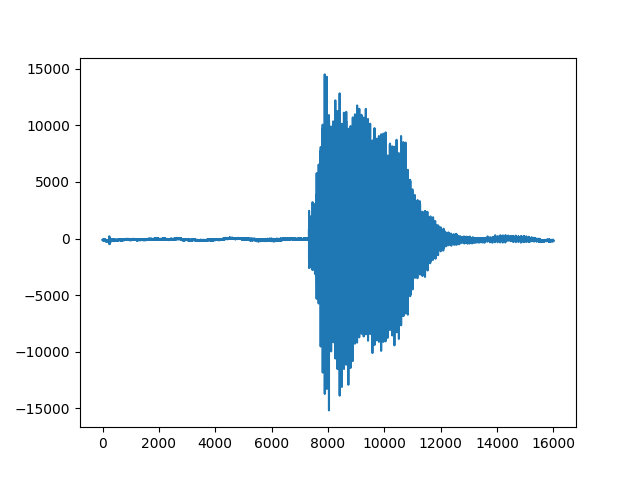
\includegraphics[width=20em]{speech_01.png}

Yapay öğrenme bağlamında zaman serileri için daha önce [7] yazısında LSTM
yapısını görmüştük. Örnek olarak zaman serilerini sınıfladık, zaman
serisindeki tüm veriler LSTM'e verilmişti, o zaman bir şeride 150 kusur
veri noktası varsa, o kadar LSTM hücresi yaratılacaktı. Fakat içinde
binlerce öğe olan seriler için bu iyi olmayabilir. Çözüm seriyi bir şekilde
özetleyerek bu daha az olan veriyi LSTM'e vermek. Bu özetlere ses işleme
alanında parmak izi (fingerprint) ismi de verilmekte.

Ses verilerini frekans üzerinden özetlemek bilinen bir teknik, ses verisi
ufak pencerelere bölünür, bu pencereler üzerinde Fourier transformu
işletilir, ve oradaki frekans bilgileri, hangi frekansın ne kadar önemli
olduğu elde edilir. Spektogram bu bilgiyi renkli olarak göstermenin bir
yolu, üstteki ses için,

\begin{minted}[fontsize=\footnotesize]{python}
plt.specgram(v[1], Fs=util.fs, NFFT=1024)
plt.savefig('speech_02.png')
\end{minted}

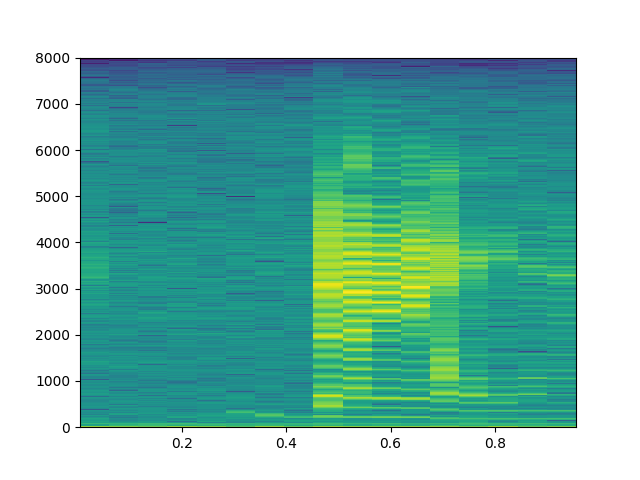
\includegraphics[width=20em]{speech_02.png}

Spektogramın örüntü tanıma için kullanılabileceğini anlamak için bir tane
daha farklı 'down' sesi, bir de 'no' sesinin spektogramına bakalım,

\begin{minted}[fontsize=\footnotesize]{python}
f1 = util.train_dir + '/down/0f3f64d5_nohash_2.wav'
wav1 = io.BytesIO(open(f1).read())
v1 = scipy.io.wavfile.read(wav1)
plt.specgram(v1[1], Fs=util.fs, NFFT=1024)
plt.savefig('speech_03.png')

f2 = util.train_dir + '/no/01bb6a2a_nohash_0.wav'
wav2 = io.BytesIO(open(f2).read())
v2 = scipy.io.wavfile.read(wav2)
plt.specgram(v2[1], Fs=util.fs, NFFT=1024)
plt.savefig('speech_04.png')
\end{minted}

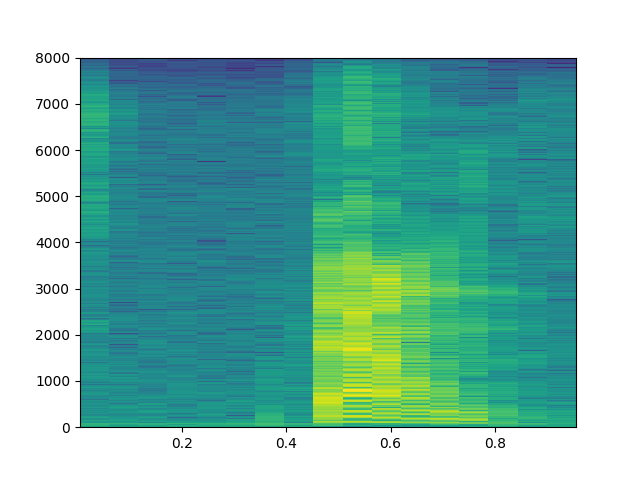
\includegraphics[width=20em]{speech_03.png}
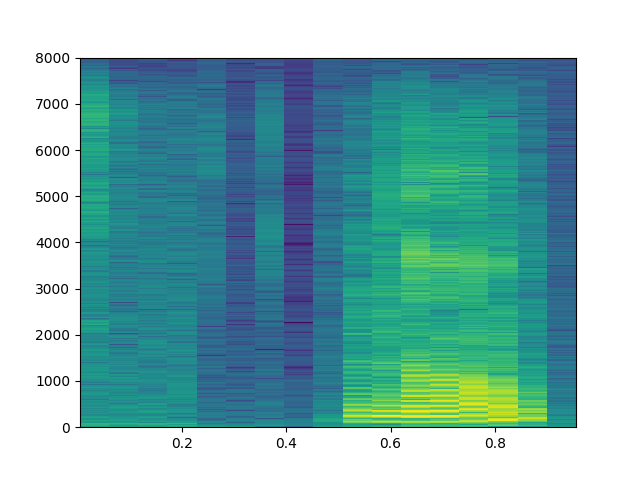
\includegraphics[width=20em]{speech_04.png}

Görüyoruz ki 'down' seslerinin spektogramları birbirine benziyor. Öğrenme
için bu yapıyı kullanabiliriz. Bu arada spektogram ``grafiği'' y-ekseninde
frekansları, x-ekseni zaman adımları gösterir, grafikleme kodu her zaman
penceresindeki belli frekans kuvvetlerinin hangi frekans kutucuğuna
düştüğüne bakar ve o kutucukta o kuvvete göre renklendirme yapar. Şimdi bu
grafikleme amaçlı, ama bazıları bu grafiğe bakarak ``ben çıplak gözle bunu
tanıyabiliyorum, o zaman görsel tanımayla üstteki imajla sesi tanıyacak bir
DYSA kullanayım'' diye düşünebiliyor. Bu işleyen bir metot, zaten DYSA'nın
görsel tanıma tarihi eski, orada bilinen bir sürü teknik var. Her neyse
bazıları üstteki görsel spektogram grafiği, yani R,G,B kanallı çıktı
üzerinde görsel tanıma yapmayı da seçebiliyor, fakat bu şart değil, bir
spektogram, bir veri durumunda iki boyutlu bir matriste gösterilebilir.
TensorFlow ile bu hesabı örnek rasgele bir veri üzerinde yapalım,

\begin{minted}[fontsize=\footnotesize]{python}
import tensorflow as tf

init_op = tf.global_variables_initializer()
data = tf.placeholder(tf.float32, [1, 16000])
print data
stfts = tf.contrib.signal.stft(data, frame_length=400, 
                               frame_step=100, fft_length=512)

spec = tf.abs(stfts)
print spec

s = np.random.rand(1,16000) # rasgele bir zaman serisi uret
with tf.Session() as sess:
     sess.run(tf.global_variables_initializer())
     res = sess.run(spec, feed_dict={data: s })  
print res
\end{minted}

\begin{verbatim}
Tensor("Placeholder_1:0", shape=(1, 16000), dtype=float32)
Tensor("Abs_1:0", shape=(1, 157, 257), dtype=float32)
[[[  99.39490509   65.10092163   12.84116936 ...,    5.39213753
      3.90902305    1.35875702]
  [ 100.60041809   66.32343292   12.92744541 ...,    4.64194965
      1.80256999    2.0458374 ]
  [ 104.70896149   70.13975525   15.93750095 ...,    3.21846962
      1.70909929    1.34316254]
  ..., 
  [  97.82588196   63.51060867   11.62135887 ...,    3.23712349
      1.94706416    0.41742325]
  [ 105.89834595   71.85715485   17.83632851 ...,    4.6476922
      2.42140603    1.37829971]
  [ 106.46664429   71.12073517   16.69457436 ...,    6.58148479
x      3.24354243    3.80913925]]]
\end{verbatim}

Cok Katmanlı LSTM

LSTM, ya da diğer her RNN çeşidi çok katmanlı olarak kullanılabilir. 

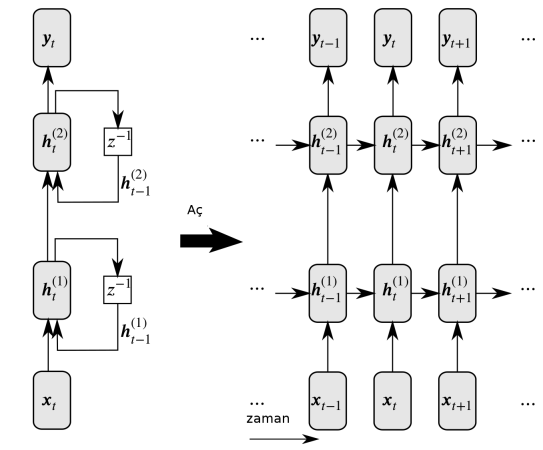
\includegraphics[width=20em]{stacked-rnn.png}

Girdiler en alttaki LSTM hücrelerine geçiliyor, bu hücreler birbirlerine
konum aktarımı yaptıkları gibi bir sonraki LSTM katmanına girdi de 
sağlıyorlar, bu aktarım en üst tabakaya kadar gidiyor. Peki o zaman
sınıflama amaçlı olarak kullanılan ``en son'' hücre hangisi olacaktır?
Bunun için tipik olarak katmanlı LSTM'de en üst ve en sondaki hücre
kullanılır. 

Her hücrede 200 nöron var, o zaman her katman (124,200) boyutunda çünkü
spektogramdan 124 zaman boyutu geldi, ve LSTM'in en sondaki hücreden alınan
vektör 200 boyutunda olacak, bu çıktı bir tam bağlanmış (fully-connected)
katmana verilerek buradan 4 tane etiket için olasılık üretilecek, ve tahmin
için kullanılan sonuçlar bunlar olacak. O sayılardan en büyük olanı en
olası olan ses komutudur.

Tüm modeli görelim,

\inputminted[fontsize=\footnotesize]{python}{model_lstm.py}

Modelin girdi tensor'un boyutlarını nasıl değiştirdiği altta (üstteki resim
iki katman gösterdi, bizim modelde 4 katman var),

\begin{minted}[fontsize=\footnotesize]{python}
import model_lstm
m = model_lstm.Model()
\end{minted}

\begin{verbatim}
Tensor("Placeholder_1:0", shape=(?, 16000), dtype=float32)
Tensor("stft/rfft:0", shape=(?, 124, 129), dtype=complex64)
Tensor("Abs:0", shape=(?, 124, 129), dtype=float32)
Tensor("rnn/transpose:0", shape=(?, 124, 200), dtype=float32)
LSTMStateTuple(c=<tf.Tensor 'rnn/while/Exit_2:0' shape=(?, 200) dtype=float32>, h=<tf.Tensor 'rnn/while/Exit_3:0' shape=(?, 200) dtype=float32>)
LSTMStateTuple(c=<tf.Tensor 'rnn/while/Exit_4:0' shape=(?, 200) dtype=float32>, h=<tf.Tensor 'rnn/while/Exit_5:0' shape=(?, 200) dtype=float32>)
LSTMStateTuple(c=<tf.Tensor 'rnn/while/Exit_6:0' shape=(?, 200) dtype=float32>, h=<tf.Tensor 'rnn/while/Exit_7:0' shape=(?, 200) dtype=float32>)
LSTMStateTuple(c=<tf.Tensor 'rnn/while/Exit_8:0' shape=(?, 200) dtype=float32>, h=<tf.Tensor 'rnn/while/Exit_9:0' shape=(?, 200) dtype=float32>)
Tensor("rnn/while/Exit_8:0", shape=(?, 200), dtype=float32)
Tensor("fully_connected/BiasAdd:0", shape=(?, 4), dtype=float32)
\end{verbatim}

Eğitim kodu,

\inputminted[fontsize=\footnotesize]{python}{train_rnn.py}

Eğitim sonrası modelin başarısı eğitim verisi üzerinde yüzde 91, doğrulama
verisinde yüzde 92. Kullanılan veri [6]'da.

Dropout

TF ile katmanlararası her noktada dropout kullanılabilir. Dropout ile bir
katmandan çıkan ya da ona giren bağlantıların bir kısmı yoksayılır, ve
model elde kalanlar ile iş yapmaya uğraşır, aşırı uygunluk problemlerinden
böylece kaçınılmış olur. Üstteki kodda hangi olasılıkla dropout
yapılacağının olasılığı bir yer tutucu (placeholder) ile TF çizitinin
parçası haline getirildi, niye? Böylece son üründeki kullanımda bu
parametre 0 yapılarak hiç dropout yapılmaması sağlanabiliyor. Eğitim
sırasında bu değer 0.5, 0.2, vs yapılabilir, o zaman dropout devrede
olur. Gerçi biz eğitim sırasında da 0 ile eğittik, yani dropout
kullanmadık, ama lazım olduğu yerler olabilir, referans açısından burada
dursun.

Uygulama

Mikrofondan 1 saniyelik ses parçalarını alıp onu model üzerinde işletip
dört komuttan birini seçen örnek kod \verb!mic.py!'da
bulunabilir. Performans gerçek zamanlı kullanım için yeterliydi, DYSA ufak
bir şey değil aslında, kaç parametre olduğuna bakalım,

\begin{minted}[fontsize=\footnotesize]{python}
print util.network_parameters(), 'tane degisken var'
\end{minted}

\begin{verbatim}
1227204 tane degisken var
\end{verbatim}

1 milyon küsur parametreli bir DYSA , yani potansiyel olarak her saniye en
az bir milyon işlem yapılıyor demektir. Görünüşe göre hesap işliyor, TF
bazı optimizasyonlar yapmış belki, ve mikroişlemciler yeterince
hızlı. Teknoloji güzel şey.

CTC

Ses tanıma için bir diğer yaklaşım optik karakter tanıma yazısında görülen
CTC kullanımı [4,5]. Alttaki kodun kullandığı veri [1]'de, yaklaşımın
detayları [2]'de görülebilir. Bu ses verisi koca kelimeler, cümleleri
içeriyor, çok daha uzun veriler bunlar, ve kayıp fonksiyonu artık basit,
belli sayıda komut arasından seçim bazlı değil, büyük bir alfabeden gelen
öğelerin yanyana gelişini kontrol ediyor.

\inputminted[fontsize=\footnotesize]{python}{train_ctc.py}

Kaynaklar

[1] Bayramlı, {\em VCTK Ses Tanima Verisi, Konusmaci 225}, \url{https://drive.google.com/uc?export=view&id=1zK-mgG6Q8N8OuOGpexbxVkES3DuQhGOk}

[2] Remy, {\em Application of Connectionist Temporal Classification (CTC) for Speech Recognition},\url{https://github.com/philipperemy/tensorflow-ctc-speech-recognition}

[3] Graves, {\em Supervised Sequence Labelling with Recurrent Neural Networks}, \url{https://www.cs.toronto.edu/~graves/preprint.pdf}

[4] Graves, {\em How to build a recognition system (Part 1): CTC Loss}, \url{https://docs.google.com/presentation/d/1AyLOecmW1k9cIbfexOT3dwoUU-Uu5UqlJZ0w3cxilkI}

[5] Graves, {\em How to build a recognition system (Part 2): CTC Loss}, \url{https://docs.google.com/presentation/d/12gYcPft9_4cxk2AD6Z6ZlJNa3wvZCW1ms31nhq51vMk}

[6] Bayramlı, {\em Ses Komut Verisi}, \url{https://drive.google.com/open?id=1BIGj3NtUZfSrXMaJ8hCqsz0UzS01MSrF}

[7] Bayramlı, Bilgisayar Bilim, {\em Uzun Kısa-Vade  Hafıza Ağları}



\end{document}
